% !TeX root = ../../Book1.tex
% 纲要标题：### 4.3 流形所需的分离与可数性
% 纲要位置：几何学计划纲要.md，第 252 行。
% 正文状态：初稿；尚未正式审核。

% 纲要内容开始
% 
% * Hausdorff、正则与正规空间
% * 第二可数和可数穷竭
% * 局部紧、第二可数 Hausdorff 空间的仿紧性
% * Urysohn 引理与正则第二可数空间的度量化
% 
% 纲要内容结束

\section{流形所需的分离与可数性}
\label{g1:sec:0403}

Euclid 空间有两种看似不同的便利：可以把一个闭集与外面的点隔开，也可以用可数个小球描述所有开集。前一种便利允许我们在邻域内部留出余地，后一种便利使全空间上的选择能够按序组织。它们结合起来，将产生紧集穷竭、局部有限覆盖和与原拓扑相容的距离。本节把这些结论的假设逐项分开；后面定义流形时采用 Hausdorff 和第二可数条件，正是为了能够使用这些整体构造。

\subsection{Hausdorff、正则与正规空间}
\label{g1:subsec:0403:01}

\cref{g1:def:hausdorff}中的 Hausdorff 条件要求不同的两个点有不交开邻域。但在构造函数时，我们常要让一个函数在整块闭集上取零，而在另一块闭集上取一；只分离两个点还不够。下面的条件依次扩大需要分离的对象。

\begin{definition}[分离条件]\label{g1:def:regular-normal}
	设 \(X\) 为拓扑空间。若每个单点集都闭，称 \(X\) 满足\term[t1kongjian]{\(T_1\) 条件}[\(T_1\) separation axiom]。本书采用以下约定。
	\begin{enumerate}
		\item 若 \(X\) 满足 \(T_1\) 条件，且对每个闭集 \(F\subseteq X\) 及每个 \(x\notin F\)，都存在不交开集 \(U,V\)，使 \(x\in U\)、\(F\subseteq V\)，则称它为\term[zhengzekongjian]{正则空间}[regular space]。
		\item 若 \(X\) 满足 \(T_1\) 条件，且任意两个不交闭集 \(A,B\subseteq X\) 都有不交开邻域，则称它为\term[zhengguikongjian]{正规空间}[normal space]。
	\end{enumerate}
\end{definition}

一些文献把上述分离性质与 \(T_1\) 条件分开命名，因此使用外部结果时需要核对约定。在本书的约定下，
\[
	\text{正规}\ \Longrightarrow\ \text{正则}\ \Longrightarrow\ \text{Hausdorff}\ \Longrightarrow\ T_1.
\]
前两个箭头分别把一个闭集取成单点、把两个闭集都取成单点。最后一个箭头来自：若 \(y\ne x\)，Hausdorff 条件给出一个含 \(y\) 而不含 \(x\) 的开邻域；这些邻域之并是 \(X\setminus\{x\}\)。

\begin{lemma}[分离与邻域缩小]\label{g1:lem:regular-normal-shrink}
	设 \(X\) 满足 \(T_1\) 条件。
	\begin{enumerate}
		\item \(X\) 正则，当且仅当对每个 \(x\in G\)（\(G\) 开），存在开集 \(V\)，使 \(x\in V\subseteq\overline V\subseteq G\)。
		\item \(X\) 正规，当且仅当对每个闭集 \(A\) 和包含它的开集 \(G\)，存在开集 \(V\)，使 \(A\subseteq V\subseteq\overline V\subseteq G\)。
	\end{enumerate}
\end{lemma}
\begin{proof}
	先看第二项。若 \(X\) 正规，对不交闭集 \(A\) 与 \(X\setminus G\) 取不交开邻域 \(V,W\)。因为 \(X\setminus W\) 闭且包含 \(V\)，有 \(\overline V\subseteq X\setminus W\subseteq G\)。反之，对不交闭集 \(A,B\)，把缩小性质用于 \(A\subseteq X\setminus B\)。所得 \(V\) 与 \(X\setminus\overline V\) 是分别包含 \(A,B\) 的不交开集。第一项的论证相同，只需把 \(A\) 换成单点 \(\{x\}\)。
\end{proof}

把闭包也留在原邻域内的缩小方式，为取极限、控制支集与零延拓留出了余地。\cref{g1:lem:local-compact-shrink}已经说明，局部紧 Hausdorff 空间具有这种点的邻域缩小性质，而且可以要求闭包紧。因此局部紧 Hausdorff 空间正则；此处尚未要求它第二可数。

\begin{example}[度量空间中的分离函数]\label{g1:exm:metric-normal}
	每个度量空间 \((X,d)\) 都正规。单点集闭；若 \(A,B\) 是非空不交闭集，令
	\[
		d(x,A)=\inf_{a\in A}d(x,a),\qquad
		h(x)=\frac{d(x,A)}{d(x,A)+d(x,B)}.
	\]
	三角不等式给出 \(|d(x,A)-d(y,A)|\le d(x,y)\)，故两个距离函数连续。又因 \(A,B\) 闭且不交，它们的距离函数不可能在同一点同时为零，所以分母处处为正。于是 \(h\) 连续，在 \(A\) 上为零，在 \(B\) 上为一；开集 \(\{h<1/3\}\) 与 \(\{h>2/3\}\) 分离 \(A,B\)。若有一个闭集为空，直接取空集和全空间即可。
\end{example}

这里没有要求两个闭集之间的距离为正。例如平面中 \(A=\{(t,0):t\ge1\}\) 与 \(B=\{(t,1/t):t\ge1\}\) 都闭，二者距离的下确界却为零。上例只需要每个固定点处的分母为正，并不需要全空间上一致的正下界。

\subsection{第二可数和可数穷竭}
\label{g1:subsec:0403:02}

为了在不同地方选择局部数据，我们希望这些选择能够列成一张可数清单。局部与整体的可数性具有不同的量词：“每一点有可数个基本邻域”允许不同的点各自使用一张清单；“全空间有可数个基本开集”要求一张清单适用于所有点。

\begin{definition}[可数性条件]\label{g1:def:countability}
	设 \(X\) 为拓扑空间。若每一点 \(x\) 都有可数邻域基，即存在含 \(x\) 的开集 \(U_1,U_2,\ldots\)，使每个含 \(x\) 的开集都包含某个 \(U_n\)，则称该空间\term[diyikeshu]{第一可数}[first countable]。若 \(X\) 的整个拓扑有一个可数基，则称它\term[dierkeshu]{第二可数}[second countable]。若 \(X\) 有可数稠密子集，称它\term[kefenkongjian]{可分}[separable]。若每个开覆盖都有可数子覆盖，称它具有\term[lindelofxingzhi]{Lindelöf 性质}[Lindelöf property]。\footnote{Ernst Leonard Lindelöf（1870--1946），芬兰数学家，研究函数论与微分方程。}
\end{definition}

可数在这里包括有限。第二可数立即蕴含第一可数：只取全空间的基中那些包含给定点的成员。每个度量空间都第一可数，因为 \(B(x,1/n)\) 构成 \(x\) 的邻域基；但一个度量空间不一定第二可数。若一个离散空间不可数，其每个单点都是开集，任何拓扑基都必须包含所有单点。

\begin{proposition}[第二可数的两项后果]\label{g1:prop:second-countable-lindelof}
	第二可数空间是可分空间，并具有 Lindelöf 性质。第二可数性遗传给任意子空间；Lindelöf 性质遗传给闭子空间。
\end{proposition}
\begin{proof}
	设 \(\{B_n\}\) 是可数基，忽略空的基元素。在每个 \(B_n\) 中取一点 \(x_n\)，所得可数点集与每个非空开集相交，因为每个这样的开集都包含某个 \(B_n\)。所以它稠密。

	给定开覆盖 \(\mathcal U\)，对每个能够包含在某个覆盖成员中的 \(B_n\)，选定一个这样的 \(U_n\in\mathcal U\)。所得至多可数个 \(U_n\) 覆盖 \(X\)：若 \(x\in U\in\mathcal U\)，基的性质给出 \(x\in B_n\subseteq U\)，于是选定的 \(U_n\) 也包含 \(x\)。

	若 \(Y\subseteq X\)，则 \(\{B_n\cap Y\}\) 是子空间的可数基。最后设 \(F\) 是 Lindelöf 空间 \(X\) 的闭子集，且 \(\{F\cap U_\alpha\}\) 是 \(F\) 的相对开覆盖，其中 \(U_\alpha\) 在 \(X\) 中开。把 \(X\setminus F\) 加入 \(\{U_\alpha\}\) 得到 \(X\) 的开覆盖，取可数子覆盖再与 \(F\) 相交即可。
\end{proof}

在 Euclid 空间中，以有理坐标点为中心、正有理数为半径的开球构成可数基。其关键不只是中心稠密，还在于可以把半径取得足够小：给定 \(x\in U\)，先取 \(B(x,\varepsilon)\subseteq U\)，再取靠近 \(x\) 的有理点 \(q\) 和满足 \(\lVert x-q\rVert<r<\varepsilon-\lVert x-q\rVert\) 的正有理数 \(r\)，便有 \(x\in B(q,r)\subseteq U\)。

\begin{definition}[紧穷竭]\label{g1:def:compact-exhaustion}
	设 \(X\) 为拓扑空间。一列紧集 \((K_n)_{n\ge1}\) 若满足
	\[
		K_n\subseteq\operatorname{int}K_{n+1},\qquad
		X=\bigcup_{n\ge1}K_n,
	\]
	称为 \(X\) 的一个\term[jinqiongjie]{紧穷竭}[compact exhaustion]。内部和闭包均在 \(X\) 中计算。
\end{definition}

\cref{g1:def:locally-compact}中的相对紧是指子集在环境空间中的闭包紧。下面会先得到由相对紧开集组成的可数基，再把这些开集分批装进紧穷竭。

\begin{theorem}[可数相对紧基与紧穷竭]\label{g1:thm:compact-exhaustion}
	局部紧、第二可数的 Hausdorff 空间 \(X\) 有可数相对紧开基，并有紧穷竭。对这样的穷竭，每个紧子集 \(C\subseteq X\) 都包含于某个 \(\operatorname{int}K_N\)。
\end{theorem}
\begin{proof}
	空空间取所有 \(K_n=\varnothing\)。以下设 \(X\ne\varnothing\)。从一个可数开基出发，只保留相对紧的基元素。它们仍是基：给定 \(x\in U\) 且 \(U\) 开，\cref{g1:lem:local-compact-shrink}给出开集 \(V\)，满足 \(x\in V\)、\(\overline V\) 紧且 \(\overline V\subseteq U\)。再选原来的基元素 \(B\) 使 \(x\in B\subseteq V\)，则 \(\overline B\) 是紧集 \(\overline V\) 的闭子集，因而紧。这里闭包包含于 \(\overline V\) 的事实也保证了 \(B\subseteq U\)。

	把保留下来的非空基元素列成 \(B_1,B_2,\ldots\)；若只有有限个，可以重复列出。令 \(K_1=\overline B_1\)。已构造 \(K_n\) 后，紧集 \(K_n\cup\overline B_{n+1}\) 可由有限个基元素 \(B_{j_1},\ldots,B_{j_s}\) 覆盖。定义
	\[
		K_{n+1}=\overline B_{j_1}\cup\cdots\cup\overline B_{j_s}.
	\]
	这是有限个紧集之并，仍紧，而且
	\[
		K_n\cup\overline B_{n+1}
		\subseteq B_{j_1}\cup\cdots\cup B_{j_s}
		\subseteq\operatorname{int}K_{n+1}.
	\]
	因此所需的内部包含关系成立，各 \(B_n\) 也都被某个 \(K_n\) 包含，故这些紧集穷尽 \(X\)。

	最后，由 \(K_n\subseteq\operatorname{int}K_{n+1}\)，开集 \(\operatorname{int}K_n\) 覆盖 \(X\)。它们递增，所以对紧集 \(C\) 取有限子覆盖后，最大的下标 \(N\) 已满足 \(C\subseteq\operatorname{int}K_N\)。
\end{proof}

紧穷竭除了满足 \(X=\bigcup_nK_n\)，还通过相邻紧集的内部包含关系留出余地。内部包含关系使 \(K_n\) 与 \(X\setminus K_{n+1}\) 之间隔着一层开邻域；下一小节将利用这层余地，让越来越远处选择的开集不再影响一个固定点附近。

\subsection{局部紧、第二可数 Hausdorff 空间的仿紧性}
\label{g1:subsec:0403:03}

在一个非紧空间上，开覆盖通常不能缩减为有限覆盖。然而粘合函数时，全空间上只有有限项并非必需：只要每个点附近实际上只有有限项出现，求和的连续性便仍是有限和的连续性。这就是局部有限条件的作用。

\begin{definition}[细化、局部有限与仿紧]\label{g1:def:locally-finite-refinement}
	设 \(\mathcal U\) 是 \(X\) 的覆盖，\(\mathcal V\) 是另一个覆盖。若每个 \(V\in\mathcal V\) 都包含于某个 \(U\in\mathcal U\)，则称新覆盖为原覆盖的\term[xihua]{细化}[refinement]。对于一族子集 \(\{A_i\}_{i\in I}\)，若每个 \(x\in X\) 都有一个只与有限个 \(A_i\) 相交的开邻域，则称这族集合是\term[jubuyouxian]{局部有限}[locally finite]的。若 \(X\) 的每个开覆盖都有局部有限开细化，称 \(X\) 为\term[fangjinkongjian]{仿紧空间}[paracompact space]。本书的仿紧性定义本身不包含 Hausdorff 条件。
\end{definition}

细化可以增加覆盖成员的数目；它要求新开集更贴合原覆盖，并不要求新覆盖是原覆盖的子族。局部有限也不同于“每个点只属于有限个成员”：后一条件只控制点本身，前一条件还控制它附近的所有点。例如 \(\{(1/(n+1),1/n):n\ge1\}\) 在 \(\mathbb R\) 中每点至多属于一个成员，却在 \(0\) 附近不是局部有限的。

\begin{lemma}[局部有限与闭包]\label{g1:lem:locally-finite-closures}
	若 \(\{A_i\}_{i\in I}\) 是拓扑空间 \(X\) 中的局部有限族，则 \(\{\overline A_i\}_{i\in I}\) 仍局部有限，并且
	\[
		\overline{\bigcup_{i\in I}A_i}=\bigcup_{i\in I}\overline A_i.
	\]
	特别地，局部有限闭集族的并是闭集；其任意子族的并也闭。
\end{lemma}
\begin{proof}
	若开集 \(N\) 与 \(\overline A_i\) 相交，取交点后利用闭包定义可知 \(N\) 也与 \(A_i\) 相交。因此一个只与有限个 \(A_i\) 相交的开邻域，也只与对应的有限个闭包相交。

	为证明右边的并闭，取 \(x\notin\bigcup_i\overline A_i\)，并取只与有限个闭包 \(\overline A_{i_1},\ldots,\overline A_{i_s}\) 相交的开邻域 \(N\)。开集 \(N\setminus\bigcup_{k=1}^s\overline A_{i_k}\) 包含 \(x\)，且与所有闭包都不交。故右边是包含 \(\bigcup_iA_i\) 的闭集，包含其闭包。反向包含逐项由 \(A_i\subseteq\bigcup_jA_j\) 得到。子族仍局部有限，最后一句随即成立。
\end{proof}

\begin{theorem}[由紧穷竭得到局部有限细化]\label{g1:thm:lch-paracompact}
	设 \(X\) 为局部紧、第二可数的 Hausdorff 空间。对 \(X\) 的每个开覆盖 \(\mathcal U\)，存在可数的局部有限开覆盖 \(\{V_j\}\)，使每个 \(\overline V_j\) 都紧，并包含于某个 \(U\in\mathcal U\)。特别地，\(X\) 仿紧。
\end{theorem}
\begin{proof}
	由\cref{g1:thm:compact-exhaustion}取紧穷竭 \((K_n)\)，并约定 \(K_{-1}=K_0=\varnothing\)。把 \(X\) 分成相互允许重叠的紧壳层
	\[
		S_n=K_n\setminus\operatorname{int}K_{n-1},
		\qquad
		G_n=\operatorname{int}K_{n+1}\setminus K_{n-2}.
	\]
	每个 \(S_n\) 紧，每个 \(G_n\) 开，而且 \(S_n\subseteq G_n\)：外侧包含来自 \(K_n\subseteq\operatorname{int}K_{n+1}\)，内侧避开 \(K_{n-2}\) 则来自 \(K_{n-2}\subseteq\operatorname{int}K_{n-1}\)。这些 \(S_n\) 覆盖 \(X\)，因为每个点第一次进入某个 \(K_n\) 时就属于 \(S_n\)。

	对每个 \(x\in S_n\)，选原覆盖成员 \(U_x\) 包含 \(x\)，再由\cref{g1:lem:local-compact-shrink}在开集 \(G_n\cap U_x\) 中缩小邻域，得到
	\[
		x\in V_x,\qquad
		\overline V_x\text{ 紧},\qquad
		\overline V_x\subseteq G_n\cap U_x.
	\]
	利用 \(S_n\) 紧，为这一层保留有限个 \(V_{n,1},\ldots,V_{n,r_n}\)。空壳层不需选择成员。所有层的选择合起来是可数开细化，并覆盖 \(X\)。

	剩下要证明的是局部有限；每层有限还不足以直接给出这个结论。给定 \(x\in X\)，选 \(m\) 使 \(x\in\operatorname{int}K_m\)。当 \(n\ge m+2\) 时，\(K_m\subseteq K_{n-2}\)，而这一层的全部 \(V_{n,k}\) 都位于 \(G_n\subseteq X\setminus K_{n-2}\)，故它们与 \(\operatorname{int}K_m\) 不交。于是该邻域只可能遇到前 \(m+1\) 层中的有限个成员，这正是局部有限。
\end{proof}

在这个构造中，\(S_n\) 是需要覆盖的区域，\(G_n\) 是允许选择邻域的稍大区域。让第 \(n\) 层避开 \(K_{n-2}\)，而不只要求它留在 \(K_{n+1}\) 以内，保证了远处的开集不会重新伸回固定点附近。

\begin{figure}[htbp]
	\centering
	% !TeX root = ../Book1.tex
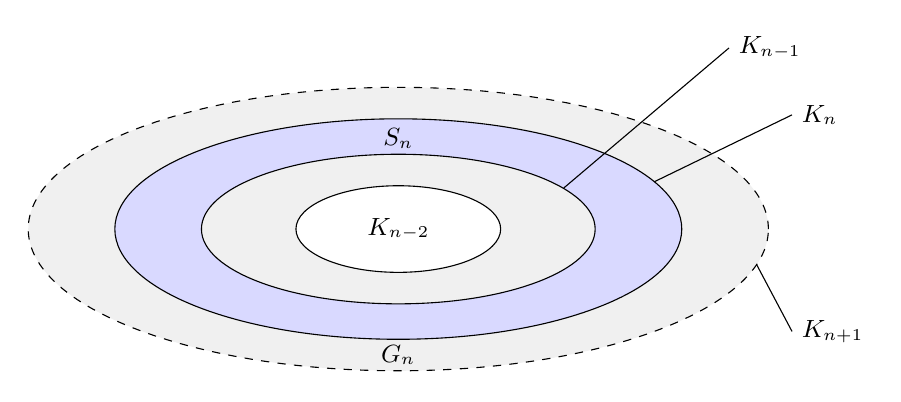
\begin{tikzpicture}[x=1cm,y=1cm,font=\small]
	\fill[gray!12,even odd rule] (0,0) ellipse (4.7 and 1.8) (0,0) ellipse (1.3 and .55);
	\fill[blue!15,even odd rule] (0,0) ellipse (3.6 and 1.4) (0,0) ellipse (2.5 and .95);
	\draw[dashed] (0,0) ellipse (4.7 and 1.8);
	\draw (0,0) ellipse (3.6 and 1.4);
	\draw (0,0) ellipse (2.5 and .95);
	\draw (0,0) ellipse (1.3 and .55);
	\node at (0,0) {\(K_{n-2}\)};
	\node at (0,1.15) {\(S_n\)};
	\node at (0,-1.6) {\(G_n\)};
	\draw (2.1,.52) -- (4.2,2.3) node[right] {\(K_{n-1}\)};
	\draw (3.25,.6) -- (5,1.45) node[right] {\(K_n\)};
	\draw (4.55,-.45) -- (5,-1.3) node[right] {\(K_{n+1}\)};
\end{tikzpicture}

	\caption{蓝色壳层 \(S_n\) 位于灰色区域 \(G_n\) 内，内外各留一层余地。曲线仅表示包含关系，并未假定空间嵌入平面。}
	\label{g1:fig:compact-exhaustion-shells}
\end{figure}

\begin{theorem}[仿紧 Hausdorff 空间的正规性]\label{g1:thm:paracompact-normal}
	每个仿紧 Hausdorff 空间都是正规空间。
\end{theorem}
\begin{proof}
	先证明正则性，不能在这一步预先使用闭包缩小。给定闭集 \(F\) 和 \(x\notin F\)，对每个 \(y\in F\)，由 Hausdorff 条件取分别含 \(x,y\) 的不交开集 \(P_y,Q_y\)。于是 \(x\notin\overline{Q_y}\)。对开覆盖
	\[
		\{X\setminus F\}\cup\{Q_y:y\in F\}
	\]
	取局部有限开细化 \(\{W_i\}_{i\in I}\)，并令 \(I_F=\{i:W_i\cap F\ne\varnothing\}\)。若 \(i\in I_F\)，则 \(W_i\) 不可能包含于 \(X\setminus F\)，所以必包含于某个 \(Q_y\)，从而 \(x\notin\overline W_i\)。由\cref{g1:lem:locally-finite-closures}，
	\[
		H=\bigcup_{i\in I_F}\overline W_i
	\]
	是一个不含 \(x\) 的闭集。于是 \(X\setminus H\) 与 \(\bigcup_{i\in I_F}W_i\) 是分别包含 \(x,F\) 的不交开集。Hausdorff 条件已保证 \(T_1\)，故 \(X\) 正则。

	现在设 \(A,B\) 是不交闭集。由刚证的正则性及\cref{g1:lem:regular-normal-shrink}，对每个 \(a\in A\) 取开集 \(O_a\)，满足 \(a\in O_a\)、\(\overline O_a\subseteq X\setminus B\)。对覆盖
	\[
		\{X\setminus A\}\cup\{O_a:a\in A\}
	\]
	再取局部有限开细化 \(\{V_j\}_{j\in J}\)。保留那些与 \(A\) 相交的成员，其下标集记为 \(J_A\)。每个这样的 \(V_j\) 必包含于某个 \(O_a\)，所以它的闭包避开 \(B\)。局部有限性保证 \(F_A=\bigcup_{j\in J_A}\overline V_j\) 闭，且仍避开 \(B\)。因此 \(\bigcup_{j\in J_A}V_j\) 与 \(X\setminus F_A\) 是 \(A,B\) 的不交开邻域，得到正规性。
\end{proof}

紧空间的每个开覆盖都有有限子覆盖，而有限族总是局部有限的。因此紧 Hausdorff 空间正规；这里紧性提供有限子覆盖，Hausdorff 条件负责最初的点分离。对流形将使用的局部紧、第二可数 Hausdorff 空间，上面两条定理则把“局部紧”转化成了整个空间上的正规性。

\subsection{Urysohn 引理与正则第二可数空间的度量化}
\label{g1:subsec:0403:04}

如果拓扑已经来自距离，\cref{g1:exm:metric-normal}用距离函数构造了取值在 \([0,1]\) 中的连续分离函数。现在反过来：先仅用开集与闭集构造足够多的这样的函数，再把函数值的差组合成距离。需要解决两个问题：如何在没有距离时构造连续函数，以及如何把全空间的分离任务缩减到可数个函数。

\begin{lemma}[正则 Lindelöf 空间的正规性]\label{g1:lem:regular-lindelof-normal}
	每个正则且具有 Lindelöf 性质的空间都是正规空间。
\end{lemma}
\begin{proof}
	设 \(A,B\) 为不交闭集。由正则性，为 \(A\) 的各点取闭包避开 \(B\) 的开邻域。闭子空间 \(A\) 仍有 Lindelöf 性质，故可取可数个这样的开集 \(U_n\) 覆盖 \(A\)。同样可取开集 \(V_n\) 覆盖 \(B\)，使 \(\overline V_n\cap A=\varnothing\)。若某一族有限或为空，可补空集写成数列。令
	\[
		U=\bigcup_{n\ge1}\left(U_n\setminus\bigcup_{i=1}^n\overline V_i\right),
		\qquad
		V=\bigcup_{n\ge1}\left(V_n\setminus\bigcup_{i=1}^n\overline U_i\right).
	\]
	括号中只减去有限个闭集，因而 \(U,V\) 都开。因为所有 \(\overline V_i\) 避开 \(A\)，\(U\) 仍包含 \(A\)；同理 \(V\) 包含 \(B\)。若某点同时落在左边第 \(n\) 项与右边第 \(m\) 项中，当 \(m\le n\) 时，左边已减去 \(\overline V_m\)，不可能属于 \(V_m\)；当 \(n\le m\) 时，右边已减去 \(\overline U_n\)，同样矛盾。因此 \(U\cap V=\varnothing\)。
\end{proof}

这个交错删去有限个闭集的构造解释了可数性的用途：第 \(n\) 个开集只需避开对方的前 \(n\) 个闭包，而任意一对下标终究有一个先后关系。若直接从每个 \(U_n\) 中减去对方所有闭包，剩下的集合未必开。

\begin{lemma}[Urysohn 引理]\label{g1:lem:urysohn}
	设 \(X\) 为正规空间，\(A,B\subseteq X\) 为不交闭集。则存在连续函数 \(f:X\to[0,1]\)，使 \(f|_A=0\)、\(f|_B=1\)。
\end{lemma}

这一结果称为\term[urysohnyinli]{Urysohn 引理}[Urysohn lemma]。\footnote{Pavel Samuilovich Urysohn（1898--1924），苏联数学家，研究一般拓扑与维数理论。}构造从安排函数的“低于某一高度的区域”入手。为保证函数连续，不同高度之间需要留出闭包包含关系。

\begin{proof}
	令 \(D=\{k/2^m:0\le k\le2^m,\ m\ge0\}\subseteq[0,1]\) 为二进有理数集。我们要为每个 \(r\in D\) 构造开集 \(U_r\)，使
	\[
		A\subseteq U_0,\qquad U_1=X\setminus B,\qquad
		\overline U_r\subseteq U_s\quad(r<s,\ r,s\in D).
	\]
	先由\cref{g1:lem:regular-normal-shrink}，为闭集 \(A\subseteq X\setminus B\) 取开邻域 \(U_0\)，满足 \(\overline U_0\subseteq U_1=X\setminus B\)。假设分母为 \(2^m\) 的各开集已经构造。对相邻的 \(r=k/2^m\) 与 \(s=(k+1)/2^m\)，在闭集 \(\overline U_r\subseteq U_s\) 之间再缩小一次，得到
	\[
		\overline U_r\subseteq U_{(r+s)/2}
		\subseteq\overline U_{(r+s)/2}\subseteq U_s.
	\]
	每一层只加入这些中间开集，旧的开集保持不变。任意两个二进有理数都出现在某个共同的有限层中，逐个使用相邻包含关系，便得到全部所需的嵌套关系。

	定义
	\[
		f(x)=\inf\bigl(\{r\in D:x\in U_r\}\cup\{1\}\bigr).
	\]
	加入 \(\{1\}\) 使这个集合总非空，所以 \(f\) 在每一点都有定义并属于 \([0,1]\)。若 \(x\in A\)，则 \(x\in U_0\)，故 \(f(x)=0\)；若 \(x\in B\)，则它不属于任何 \(U_r\)，故 \(f(x)=1\)。

	下面分别检验函数值低于和高于给定高度的集合开。对 \(0<a\le1\)，下确界的性质给出
	\[
		\{f<a\}=\bigcup_{\substack{r\in D\\r<a}}U_r.
	\]
	对 \(0\le a<1\)，则有
	\[
		\{f>a\}=\bigcup_{\substack{r\in D\\a<r<1}}(X\setminus\overline U_r).
	\]
	为核对第二式，若 \(x\notin\overline U_r\)，则它不属于任何 \(U_t\)（\(t<r\)），所以 \(f(x)\ge r>a\)。反之，若 \(f(x)>a\)，取二进有理数 \(a<r<f(x)\)。若 \(x\in\overline U_r\)，则对每个二进有理数 \(s>r\) 都有 \(x\in U_s\)，从而 \(f(x)\le r\)，矛盾。故 \(x\notin\overline U_r\)。这证明第二式。上述两个集合都开；当 \(a\) 在其余范围时，它们是空集或全空间。实数开区间的原像由这两类集合相交得到，故 \(f\) 连续。
\end{proof}

若映射 \(F:X\to Y\) 是 \(X\) 到其像 \(F(X)\) 的同胚，其中像赋予 \(Y\) 的子空间拓扑，就称 \(F\) 为\term[tuopuqianru]{拓扑嵌入}[topological embedding]。下面将用可数个连续函数把原空间实现为一个可数积空间的子空间。

\begin{theorem}[Urysohn 度量化定理]\label{g1:thm:urysohn-metrization}
	设 \(X\) 为正则、第二可数的拓扑空间。则存在一列连续函数 \(f_n:X\to[0,1]\)，使
	\begin{equation}\label{g1:eq:urysohn-metric}
		d(x,y)=\sum_{n=1}^{\infty}2^{-n}|f_n(x)-f_n(y)|
	\end{equation}
	成为 \(X\) 上的度量，并且它所诱导的拓扑恰好等于原拓扑。映射 \(x\mapsto(f_n(x))_{n\ge1}\) 将 \(X\) 拓扑嵌入带积拓扑的 \([0,1]^{\mathbb N}\)。
\end{theorem}

若一个空间的拓扑可由某个距离诱导，就称这个空间\term[kelianghua]{可度量化}[metrizable]；并不预先指定距离，也不保证这个距离完备。上述结果称为\term[urysohndulianghua]{Urysohn 度量化定理}[Urysohn metrization theorem]。这里正则性含 \(T_1\) 条件。定理比“局部紧、第二可数 Hausdorff 空间可度量化”更一般，因为它不要求局部紧。

\begin{proof}
	空空间的结论按空映射成立。设 \(X\ne\varnothing\)，取可数开基 \(\{B_i\}\)。由\cref{g1:prop:second-countable-lindelof,g1:lem:regular-lindelof-normal}，\(X\) 正规。对每一对满足 \(\overline B_i\subseteq B_j\) 的下标 \((i,j)\)，把\cref{g1:lem:urysohn}用于不交闭集 \(X\setminus B_j\) 与 \(\overline B_i\)，得到连续函数 \(f_{ij}:X\to[0,1]\)，满足
	\[
		f_{ij}=1\text{ 于 }\overline B_i,\qquad
		f_{ij}=0\text{ 于 }X\setminus B_j.
	\]
	这些下标对至多可数。列出全部所得函数，并在必要时补上常值零函数，记成 \((f_n)_{n\ge1}\)。

	这些函数具有比“分开两个点”更强的性质：若 \(x\in O\) 且 \(O\) 开，可以找到一个 \(f_k\)，使 \(f_k(x)=1\)，并在 \(X\setminus O\) 上为零。事实上，先取基元素 \(x\in B_j\subseteq O\)，再由正则性选 \(x\in V\subseteq\overline V\subseteq B_j\)，最后取 \(x\in B_i\subseteq V\)。于是 \(\overline B_i\subseteq B_j\)，所对应的 \(f_{ij}\) 就满足要求。特别地，对 \(x\ne y\)，因 \(T_1\) 条件使 \(X\setminus\{y\}\) 开，这一性质给出某个 \(f_k(x)=1\)、\(f_k(y)=0\)。

	现在用\eqref{g1:eq:urysohn-metric}定义 \(d\)。每项不超过 \(2^{-n}\)，故级数收敛。对称性与非负性逐项成立；刚证的点分离性质保证 \(x\ne y\) 时 \(d(x,y)>0\)。每个函数值差满足实数的三角不等式，把前 \(N\) 项相加再令 \(N\to\infty\)，得到 \(d(x,z)\le d(x,y)+d(y,z)\)。所以 \(d\) 是度量。

	还必须证明原来的开集与度量开集相同，单有点分离并不能保证这一点。给定 \(x\in X\) 与 \(\varepsilon>0\)，取 \(N\) 使 \(\sum_{n>N}2^{-n}<\varepsilon/2\)。由前 \(N\) 个函数的连续性，存在原拓扑中的开邻域 \(V\ni x\)，使对 \(y\in V\) 及 \(1\le n\le N\)，都有 \(|f_n(x)-f_n(y)|<\varepsilon/2\)。于是前 \(N\) 项之和小于 \(\varepsilon/2\)，尾项之和也小于 \(\varepsilon/2\)，故 \(V\subseteq B_d(x,\varepsilon)\)。这说明从原拓扑到度量拓扑的恒等映射连续。

	反过来，给定原拓扑的开邻域 \(O\ni x\)，取上述满足 \(f_k(x)=1\) 且在 \(X\setminus O\) 上为零的函数。如果 \(d(x,y)<2^{-k-1}\)，则
	\[
		2^{-k}|f_k(x)-f_k(y)|\le d(x,y)<2^{-k-1},
	\]
	所以 \(f_k(y)>1/2\)，从而 \(y\in O\)。因此 \(B_d(x,2^{-k-1})\subseteq O\)，另一方向的恒等映射也连续。

	最后，令 \(F(x)=(f_n(x))\)。它由点分离性质单射，而在立方体 \([0,1]^{\mathbb N}\) 上，
	\[
		D(s,t)=\sum_{n\ge1}2^{-n}|s_n-t_n|
	\]
	是一个度量，且 \(D(F(x),F(y))=d(x,y)\)。这个度量给出积拓扑：其开球包含由有限个坐标的小变化所确定的基本开邻域，理由正是上面的尾项估计；反过来，对规定有限个坐标的邻域，取球半径小于各坐标容许变化量乘以对应 \(2^{-n}\) 的最小值，整个球便包含于该邻域。因此 \(F\) 是 \(X\) 到其像的同胚，即所称的拓扑嵌入。
\end{proof}

可以把 \((f_n(x))\) 看作一列连续测量值。正则性与 Urysohn 引理保证：无论给点 \(x\) 指定多小的开邻域，总有一项测量在 \(x\) 取一、在邻域外取零。第二可数性把所有这种局部区分压缩为可数个测量；权重 \(2^{-n}\) 则让后面无穷多项的总影响可以统一控制。

\begin{corollary}[流形所用的拓扑结论]\label{g1:cor:lch-second-countable}
	每个局部紧、第二可数的 Hausdorff 空间都可度量化、仿紧且正规，并具有紧穷竭。
\end{corollary}
\begin{proof}
	局部紧 Hausdorff 空间由邻域缩小性质正则，因此可应用\cref{g1:thm:urysohn-metrization}。紧穷竭、仿紧性与正规性分别由\cref{g1:thm:compact-exhaustion,g1:thm:lch-paracompact,g1:thm:paracompact-normal}得到。
\end{proof}

这个推论给出与开集相容的点间距离，式\eqref{g1:eq:urysohn-metric}中的距离未必完备。Riemann 度量则在每个切空间上指定随点光滑变化的内积；下一节的连续单位分解将先说明这类局部数据怎样加权粘合。
